\documentclass{article}
\usepackage{setspace} 
\usepackage{graphicx}
\addtolength{\topmargin}{-.575in}
\addtolength{\textheight}{1.25in}


\usepackage{Sweave}
\begin{document}
\Sconcordance{concordance:lit_review.tex:lit_review.Rnw:%
1 7 1 1 0 51 1}


\begin{spacing}{1.5}
\phantom
\phantom
\section*{Chapter 2 \\ \huge{Literature Review}}
\phantom
\phantom
The boreal forest of Canada are one of the world's largest stores of carbon, provide a vast array of ecosystem services, and are home to valuable biological diversity. The forest have also played a prominent role in Canada's social and economic development (Drushka, 2003). It is therefore, no wonder that public fire management agencies expend great deal of effort and resources fighting the seasonal wildfires that threaten this valuable resource (Martell 2001). In the fire management literature, it has long been assumed that these fire suppression efforts are effective (Cumming 2005:772). However, in recent years, fire ecologists have begun to question the received wisdom (Miyanishi {\it et al}. 2002). \\

The case for effective fire suppression rests on a number of retrospective comparisons between forest regions in Ontario, Canada (Stocks 1991, Ward and Tithecott 1993; Martell 1994; Ward {\it et al.} 2001). These studies compared the size distributions of forest fires in areas with and without aggressive fire suppression policies, in order to measure the effectiveness of fire suppression at reducing the annual area of forest burned (Cumming 2005:772-773). The results revealed a highly right-skewed distribution in areas with aggressive fire suppression and a relatively flat distribution in areas without such policies. The authors concluded that fire suppression had been successful at reducing the annual area burned over recent decades (Bridge {\it et al.} 2005:43). \\

However, Miyanishi {\it et al.} (2002; also see Johnson {\it et al.} 2001; Miyanishi and Johnson 2001) argue that these studies failed to control for various spatial and temporal factors, (e.g. the underlying fire-size distributions, the fire-detection efficiency and the probability that small fires are recorded), which have been shown to distort the results of similar studies, and on that basis should be considered unsound. \\

While both parties agree that fire suppression is primarily intended to reduce the annual area of forest burned, neither have been able to established a workable definition of fire suppression 'effectiveness' (Cumming 2005:781). Cumming (2005:773) has argued that a definition of 'effectiveness' only requires that annual burn rates with aggressive fire suppression be lower than they would have been without it. \\

\begin{figure}[h!]
  \centering
    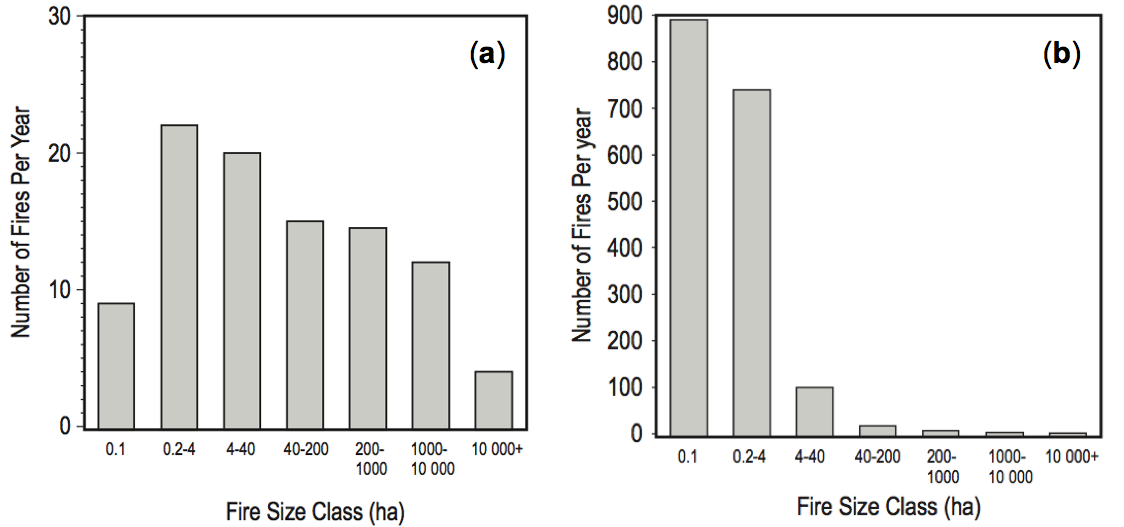
\includegraphics[width=1\textwidth]{fig1}
      \caption{Frequency distribution of fires by size class for {\bf a}) the Intensive and Measured protection zones, and {\bf b}) for the Extensive protection zones in Ontario, Canada (from Ward and Tithecott 1993).}
\end{figure}

\end{spacing}
\clearpage
\section*{References}
\phantom
\noindent Bridge, S.R.J., Miyanishi, K. and Johnson, E.A. 2005. A Critical Evaluation of Fire Suppression Effects in the Boreal Forest of Ontario. {\it Forest Science}, 51(1), 41-50.\\

\noindent Cumming, S.G. 2005. Effective fire suppression in boreal forests. {\it Canadian Journal of Forest Research}, 35(4), 772-786.\\ 

\noindent Hirsch, K.G., Corey, P.N., and Martell, D.L. 1998. Using expert judgment to model initial attack fire crew effectiveness. {\it Forest Science}, 44, 539-549.\\

\noindent Johnson, E.A., Miyanishi, K. and Bridge, S.R.J., 2001. Wildfire Regime in the Boreal Forest and the Idea of Suppression and Fuel Buildup. {\it Conservation Biology}, 15(6), 1554-1557.\\

\noindent Martell, D.L. 1994. The impact of fire on timber supply in Ontario. {\it The Forestry Chronicle}, 70, 164-173.\\

\noindent Martell, D.L. 2001. Forest fire management. In {\it Forest Fires: behavior and ecological effects}. E.A. Johnson and K. Miyanishi (Eds). San Diego, California: Academic Press, 572-583.\\

\noindent Miyanishi, K., and Johnson, E.A. 2001. A re-examination of the effects of fire suppression in the boreal forest. {\it Canadian Journal of Forest Research}, 31, 1462-1466.\\

\noindent Miyanishi, K., Bridge, S.R.J., and Johnson, E.A. 2002. Wildfire regime in the boreal forest. {\it Conservation Biology}, 16(5), 1177-1178.\\

\noindent Ontario Ministry of Natural Resources / Minist\'{e}re des Richesses Naturelles (OMNR). 1997. {\it Ontario's fire management strategies: Background, current state, and future challenges}. Toronto, Canada.\\

\noindent Strauss, D., Bednar, L., and Mees, R. 1989. Do one percent of forest fires cause ninety-nine percent of the damage? {\it Forest Science}, 35(2), 319-328.\\

\noindent Ward, P.C., and Tithecott, A.G. 1993. {\it Impact of fire management on the boreal landscape of Ontario}. Ministry of Natural Resources, Aviation, Flood and Fire Management Branch, Sault Sainte, Marie, Ontario, 305.\\

\noindent Ward, P.C., Tithecott, A.G., and Wotton, B.M. 2001. Reply-A re-examination of the effects of fire suppression in the boreal forest. {\it Canadian Journal of Forest Research}, 31, 1467-1480.\\ 

\end{document}
